\documentclass[12pt, a4paper]{report}
%\usepackage{tgtermes} % for times romans font
\usepackage{float}
\usepackage{natbib}
\usepackage{amsmath}
\usepackage{comment}
\usepackage{graphicx}
\usepackage{etoolbox}
\usepackage{hyperref}
\usepackage{geometry}
\usepackage{fancyhdr}
\usepackage{amsfonts}
\usepackage{tocbibind} % adds 'Contents' to TOC
\usepackage[T1]{fontenc}
\usepackage[utf8]{inputenc} % use utf8x if utf8 causes error
\usepackage[UKenglish]{babel}
\usepackage[section]{placeins}
\usepackage[dvipsnames]{xcolor}

\begin{comment}
    mkdir build
    pdflatex -output-directory=build main.tex
    bibtex build/main
    pdflatex -output-directory=build main.tex
    pdflatex -output-directory=build main.tex
\end{comment}

\hypersetup{
  colorlinks      = true,
  urlcolor        = brown,
  linkcolor       = black,
  citecolor       = black,
  citebordercolor = red,
  urlbordercolor  = white,
  linkbordercolor = blue,
}

\graphicspath{{../images/}}
\setlength{\headheight}{32pt}
\setcitestyle{open={},close={},numbers}
\AtBeginDocument{\hypersetup{pdfborder={0 0 1}}}

\title{\textbf{Vudoku - Visual Sudoku Solver} \\ \vspace{1cm} \large A project report submitted to APJ Abdul Kalam Technological University in partial fulfillment of the requirements for the award of the degree of \\ \vspace{0.5cm} \large \textbf{Bachelor of Technology \\ in \\ Computer Science and Engineering} \\ \vspace{0.5cm} \large by}
\author{\textbf{Jovial Joe Jayarson (IES17CS016)}}

%>>>>>>>>>>>>>>>>>>>>>>> Header & Footer >>>>>>>>>>>>>>>>>>>>>>>
\makeatletter
\patchcmd{\f@nch@head}{\rlap}{\color{gray}\rlap}{}{}
%\patchcmd{\headrule}{\hrule}{\color{gray}\hrule}{}{}
\patchcmd{\f@nch@foot}{\rlap}{\color{gray}\rlap}{}{}
%\patchcmd{\footrule}{\hrule}{\color{gray}\hrule}{}{}
\makeatother

\pagestyle{fancy}
\fancyhf{}
\lhead{Department of CSE}
\rhead{Project Report 2020-21}
\lfoot{IES College of Engineering}
\rfoot{\thepage}
\renewcommand{\headrulewidth}{0pt}
\renewcommand{\footrulewidth}{0pt}
%<<<<<<<<<<<<<<<<<<<<<<< Header & Footer <<<<<<<<<<<<<<<<<<<<<<<


%#################################################################
%                      Document Begins Here                      %
%#################################################################
\begin{document}

\newgeometry{left=3cm,right=3cm,top=3cm,bottom=3cm}

%>>>>>>>>>>>>>>>>>>>>>>> Title >>>>>>>>>>>>>>>>>>>>>>>
\makeatletter
\thispagestyle{empty}
\begin{titlepage}
    \begin{center}
        \vspace*{\fill}
        {\huge \@title }\\[0.5cm]
        {\@author} \\[0.5cm]
        {\@date}\\[10ex]
        
\includegraphics[width=0.5\linewidth]{iesce.png}\\[10ex]
        {\large Department of Computer Science and Engineering \\ \textbf{IES College of Engineering, Chittilappilly - 680551}}
        \vspace*{\fill}
    \end{center}
\end{titlepage}
%<<<<<<<<<<<<<<<<<<<<<<< Title <<<<<<<<<<<<<<<<<<<<<<<

\pagenumbering{roman}

%>>>>>>>>>>>>>>>>>>>>>>> Certificate >>>>>>>>>>>>>>>>>>>>>>>
\newpage
\thispagestyle{plain}
\vspace*{\fill}
\begin{center}
    \textbf{\textsc{IES College of Engineering}}\\[0.5cm]
    \textbf{\textsc{Department of Computer Science and Engineering}}\\[1cm]
    
\includegraphics{iesce.png}
    \section*{Certificate}
    \addcontentsline{toc}{chapter}{Certificate}
    This is to certify that the project report entitled \\[0.3cm] \textbf{\large Vudoku - Visual Sudoku Solver} \\[0.3cm] submitted by \\[0.3cm] \textbf{Jovial Joe Jayarson} \\[0.3cm] in partial fulfilment of the requirements of the degree of \emph{Bachelor of Technology in Computer Science and Engineering}, to APJ Abdul Kalam Technological University is a record of \emph{bona fide}  work done by him under my supervision and guidance and this work has not been submitted elsewhere for any degree or diploma. \\[2cm]
\end{center}

\begin{table}[h]
    \centering
    \begin{tabular}{ c c c c }
              &                    & \rule{5cm}{0.15mm}   & \rule{5cm}{0.15mm}     \\
        Place & \rule{2cm}{0.15mm} & Mr. Ebin P M         & Dr. Kiruthiga G        \\
              &                    & Asst. Professor, CSE & Head of the Department \\
        Date  & \rule{2cm}{0.15mm} & (Guide)              & CSE                    \\
    \end{tabular}
\end{table}
\vspace*{\fill}
%<<<<<<<<<<<<<<<<<<<<<<< Certificate <<<<<<<<<<<<<<<<<<<<<<<

%>>>>>>>>>>>>>>>>>>>>>>> Acknowledgement >>>>>>>>>>>>>>>>>>>>>>>
\newpage
\vspace*{\fill}
\begin{center}
    \section*{Acknowledgements}
    \addcontentsline{toc}{chapter}{Acknowledgements}
\end{center}

I gladly present this report on \emph{Vudoku - Visual Sudoku Solver} as a part of the final year B.Tech Computer Science and Engineering seminar. Let me take opportunity to first thank God the Almighty for providing His grace and guidance in this dispensation. I express my sincere thanks to Dr. Brilly S Sangeetha, principal for providing us with all the facilities we required to make this happen. I also acknowledge the ever encouraging presence of Dr. Kriuthiga G, head of the department. Heartfelt gratitude to my guide Mr. Ebin P M, Assistant Professor, for his undivided attention, support and coaching. Last but not the least I convey my regards to all the well wishers, family and friends who have helped me during the needed times.

\begin{center}
    May God bless us all.
\end{center}
\vspace*{\fill}
%<<<<<<<<<<<<<<<<<<<<<<< Acknowledgement <<<<<<<<<<<<<<<<<<<<<<<

%>>>>>>>>>>>>>>>>>>>>>>> Abstract >>>>>>>>>>>>>>>>>>>>>>>
\newpage
\vspace*{\fill}
\begin{center}
    \section*{Abstract}
    \label{sec:abstract}
    \addcontentsline{toc}{chapter}{Abstract}
\end{center}
It is no secret that AI is an upcoming titan. Even though people are stunned to hear that AI has been here for around a century, due to the advancement in computational methods and resources AI peaks like never before. As a tiny glimpse into the field of Digit Recognition, this project aims to understand the underlying cogs and wheels on which the neural networks spin. Ranging from core mathematical functions to flowery programming, this project will include all that is essential to recognize a digit from an image. Even though the project is primarily research oriented, on the application part of it, this can be used to identify licence plate, read bank cheques, grade primary class mathematics homework. Currently the project tries to solve Sudoku drawn and written by hand The paraphernalia for this project includes programming language: Python3/Nim; libraries: opencv, pandas, numpy, keras/tensorflow, matplotlib; datasets: MNIST handwritten digit database. Digit recognition is a classical problem which will introduce neurons, neural networks, connections hidden layers, weights, biases, activation functions like sigmoid and ReLU, back-propagation and other topics as well.
\vspace*{\fill}
%<<<<<<<<<<<<<<<<<<<<<<< Abstract <<<<<<<<<<<<<<<<<<<<<<<

{
    \hypersetup{hidelinks}

    \tableofcontents
    \thispagestyle{fancy}

    \listoffigures
    \thispagestyle{fancy}

    %\listoftables
    %\thispagestyle{fancy}
}

%>>>>>>>>>>>>>>>>>>>>>>> Introduction >>>>>>>>>>>>>>>>>>>>>>>
%>>>>>>>>>>>>>>>>>>>>>>> Introduction >>>>>>>>>>>>>>>>>>>>>>>
\chapter{Introduction}
\label{chap:introduction}
\pagenumbering{arabic}
\thispagestyle{fancy}

\hspace{0.5cm} Digit Recognition is a classical machine learning problem. The objective is implicitly evident, it is to identify and classify (usually) handwritten digits. Machines are inherently incapable to understand, text, images and audio. These formats which carry information, needs to be converted into numbers, matrices or vectors which is a significant step, in any procedure, to solve problems using computers. Another vital stage for digit recognition is \emph{machine learning}. With classical problem solving techniques, humans provide computers with both data and rules as input. In contrast, we provides data and presumed result, as input to a machine learning system. And then we let it find out some \emph{rules}. A quick example would be to give three numbers $x$, $y$ and $z$ and tell a machine that - certain operation was performed on $x$ and $y$ to obtain $z$. Once a machine is fed with lots and lots of similar examples, it will be equipped find out some pattern behind it. At a later stage, it can very well predict, what operation(s) might have been performed on $x$ and $y$ to result in $z$.

This report delves into a century long history of digit recognition, all the way from perceptron networks to recently released transformers. The means and ways, in which this problem was approached converges to SOTA (state of the art) models like in \cite{art:edrdcnn}. This report explores \emph{The Transformer}, released in 2017. \emph{Attention} mechanism in the Transformer \cite{2017arXiv170603762V} has sparked a lot of interest in the research community, not to mention the buzz associated with GPT-3, due to its mind-boggling capabilities flaunted all across the media. The very next year a preprint on \emph{Image Transformer} \cite{2018arXiv180205751P} was released. Interestingly Google research just released another preprint which dubs the whole idea of manipulating images with this new technique as \emph{Vision Transformer} \cite{2020arXiv201011929D}. Now at the core of this project, the digit recognition makes use of the Vision Transformer.

The project is named \emph{Vudoku}, so the second part of the project involves solving classical computational problem. Sudoku is a mathematical problem and by default has $9\times 9$ grids. There are other variant to it but to keep things simple, the project moves along with the default one. Sudoku is classified as Exact Cover or Hitting Set problem \cite{wiki:exactcover}. Various algorithms has been developed over the years to solve it, like Backtracking, Stochastic algorithms, Constraint programming and so on. Given that the output of the digit recognition system is as \emph{value}, \emph{position} pairs, this project will consider some of these algorithms to solve sudoku and possibly visualize the steps.
\vspace*{\fill}
%<<<<<<<<<<<<<<<<<<<<<<< Introduction <<<<<<<<<<<<<<<<<<<<<<<

%>>>>>>>>>>>>>>>>>>>>>>> Overview >>>>>>>>>>>>>>>>>>>>>>>
%>>>>>>>>>>>>>>>>>>>>>>> Overview >>>>>>>>>>>>>>>>>>>>>>>
\chapter{Overview and Prerequisites}
\label{chap:overview}
\thispagestyle{fancy}

\section{Overview of the Topic}
\label{sec:ovrtpc}

\hspace{0.5cm} Complex problems exists all around us. Some of them are stumbled upon and other have be thoughtfully crafted. Solutions to these problems at times are intuitive and yet difficult to explain. Structured mathematical approach to problems has engineered some of the finest solutions to some of the toughest problem. In the era of computing, appetite to solve problems using machines has become a hobby. With technology at fingertips, it's no-brainer that upcoming generations have a choice to be way smarter.

Speaking of generations, there are puzzles and trivia question that people like to solve. These are not always driven by any particular motive. Sudoku is a famous mathematical puzzle. The rules to solve this can be summarized as: \emph{All grids must be filled with numbers from 1 to 9 without repetition in either row, column or box}. Today any computer can solve this within seconds - if given with proper parameters. But computers by default do not possess visual perception. This is where image recognition steps in. This project can be thought of as an amalgamation of machine learning and classical computing. Instead of feeding a system with direct sudoku \emph{clues}, an image of sudoku is provided. The computer has to derive the clues out of an image and then pass them along with correct positions to the second modules which then tries to solve sudoku.

\section{Prerequisites for the Project}
\label{sec:prereq}

\hspace{0.5cm} Since this project strives to reach minimum research standard, reader is advised to have knowledge about related topics. This section tries to cover some of them but the rest is left at reader's discretion to follow up.

\subsection{Mathematics to solve Sudoku}
\label{subsec:mpf}

\subsubsection{NP-Complete}
In computational complexity theory, a problem is NP-complete when:
\begin{itemize}
    \item A nondeterministic Turing machine can solve it in polynomial-time.
    \item A deterministic Turing machine can solve it in large time complexity classes and can verify its solutions in polynomial time.
    \item It can be used to simulate any other problem with similar solvability. \cite{wiki:npcmpt}
\end{itemize}

\subsubsection{Combinatorics}
Combinatorics is an area of mathematics primarily concerned with counting, both as a means and an end in obtaining results \cite{wiki:combt}.

\subsubsection{Group Theory}
\label{subsec:combnt}
In mathematics and abstract algebra, group theory studies the algebraic structures known as groups. In mathematics, a group is a set equipped with a binary operation that combines any two elements to form a third element in such a way that four conditions called group axioms are satisfied, namely `closure', `associativity', `identity` and `invertibility' \cite{wiki:grpt} \cite{wiki:grps}.

\subsection{Machine Learning and related Terminology}
\label{mlrt}

\subsubsection{Gradient Descent}
Gradient descent is a first-order iterative optimization algorithm for finding a local minimum of a differentiable function. The idea is to take repeated steps in the opposite direction of the gradient (or approximate gradient) of the function at the current point, because this is the direction of steepest descent. Conversely, stepping in the direction of the gradient will lead to a local maximum of that function; the procedure is then known as gradient ascent. \cite{wiki:grdsc}.

\subsubsection{Fourier Transform}
In mathematics, a Fourier transform (FT) is a mathematical transform that decomposes a function (often a function of time, or a signal) into its constituent frequencies, such as the expression of a musical chord in terms of the volumes and frequencies of its constituent notes. The term Fourier transform refers to both the frequency domain representation and the mathematical operation that associates the frequency domain representation to a function of time \cite{wiki:fortrsfm} This is used in image preprocessing step in CNN \ref{subsec:objrecfund}.

\subsubsection{Activation Function}
In artificial neural networks, the activation function of a node defines the output of that node given an input or set of inputs. A standard integrated circuit can be seen as a digital network of activation functions that can be ``ON'' or ``OFF'', depending on input. \cite{wiki:actfnc}

\vspace*{\fill}
%<<<<<<<<<<<<<<<<<<<<<<< Overview <<<<<<<<<<<<<<<<<<<<<<<

%>>>>>>>>>>>>>>>>>>>>>>> Literature >>>>>>>>>>>>>>>>>>>>>>>
%>>>>>>>>>>>>>>>>>>>>>>> Literature >>>>>>>>>>>>>>>>>>>>>>>
\chapter{Literature Review}
\label{chap:literature}
\thispagestyle{fancy}

\section{Handwritten Digit Recognition Using Machine Learning : A Review}
\label{sec:litppr3}

\textbf{Abstract (as is)}: The task for handwritten digit recognition has been troublesome due to various variations in writing styles. Therefore, we have tried to create a base for future researches in the area so that the researchers can overcome the existing problems. The existing methods and techniques for handwritten digit recognition were reviewed and understood to analyze the most suitable and best method for digit recognition. A number of 60,000 images were used as training sets of images with pixel
size of $28\times 28$. The images/training sets were matched with original image. It was found out after complete analysis and review that classifier ensemble system has the least error rate of
just 0.32\%. In this paper, review of different methods handwritten digit recognition were observed and analyzed.

\section{An ensemble of simple convolutional neural network models for MNIST digit recognition}
\label{sec:litppr4}

\textbf{Abstract (as is)}: We report that a very high accuracy on the MNIST test set can be achieved by using simple convolutional neural network (CNN) models. We use three different models with $3\times 3$, $5\times 5$, and $7\times 7$ kernel size in the convolution layers. Each model consists of a set of convolution layers followed by a single fully connected layer. Every convolution layer uses batch normalization and ReLU activation, and pooling is not used. Rotation and translation is used to augment training data, which is frequently used in most image classification tasks. A majority voting using the three models independently trained on the training data set can achieve up to 99.87\% accuracy on the test set, which is one of the state-of-the-art results. A two-layer ensemble, a heterogeneous ensemble of three homogeneous ensemble networks, can achieve up to 99.91\% test accuracy. The results can be reproduced by using the code at \url{https://github.com/ansh941/MnistSimpleCNN}.

\section{An Image is Worth 16x16 Words : Transformers For Image Recognition at Scale}
\label{sec:litppr5}

\textbf{Abstract (as is)}: While the Transformer architecture has become the de-facto standard for natural language processing tasks, its applications to computer vision remain limited. In vision, attention is either applied in conjunction with convolutional networks, or used to replace certain components of convolutional networks while keeping their overall structure in place. We show that this reliance on CNNs is not necessary and a pure transformer applied directly to sequences of image patches can perform very well on image classification tasks. When pre-trained on large amounts of data and transferred to multiple mid-sized or small image recognition benchmarks (ImageNet, CIFAR-100, VTAB, etc.), Vision Transformer (ViT) attains excellent results compared to state-of-the-art convolutional networks while requiring substantially fewer computational resources to train.
\vspace*{\fill}
%<<<<<<<<<<<<<<<<<<<<<<< Literature <<<<<<<<<<<<<<<<<<<<<<<

%>>>>>>>>>>>>>>>>>>>>>>> Evolution >>>>>>>>>>>>>>>>>>>>>>>
%>>>>>>>>>>>>>>>>>>>>>>> Evolution >>>>>>>>>>>>>>>>>>>>>>>
\chapter{Evolution of Neural Networks}
\label{chap:evolution}
\thispagestyle{fancy}

\hspace{0.5cm} It's of no surprise that the field of artificial intelligence has come a long way. This section deals with some of the famous models and how they are related to digit recognition. Starting from the ones released in 80's like \emph{Recurrent Neural Network (RNN)} to the latest 2017 model \emph{The Transformer}, much study has been conducted.

\section{Recurrent Neural Network}
\label{sec:RNN}

\textbf{Year:} 1986

Recurrent neural networks are derived from feed-forward networks. The connections in a feed-forward network do not form a cycle. RNN is a class of neural network where the connections between nodes form a directed graph. This is always along a temporal sequence, so it exhibits a temporal dynamic behaviour. Dynamic systems are those that have a function which describes time dependence of a point in geometrical space. RNNs can use their internal state (or memory) to process variable length sequences of inputs \cite{wiki:rnns}. Section \ref{sec:perceptron} discusses more about vanilla networks.

Basic RNNs are a network of neuron-like nodes organized into successive layers. Each node in a given layer is connected with a directed (one-way) connection to every other node in the next successive layer. Each node (neuron) has a time-varying real-valued activation. Each connection (synapse) has a modifiable real-valued weight. Nodes are either input nodes (receiving data from outside of the network), output nodes (yielding results), or hidden nodes (that modify the data en route from input to output). Each sequence produces an error as the sum of the deviations of all target signals from the corresponding activations computed by the network. For a training set of numerous sequences, the total error is the sum of the errors of all individual sequences. The following equation \ref{equ:4.1} was proposed by \textbf{Michael Irwin Jordan} as part of his research on \emph{Simple Recurrent Neural Network} \cite{wiki:rnns}:

\[h_t = \sigma_h(W_h x_t + U_h y_{t-1} + b_h)\]
\begin{equation}
    \label{equ:4.1}
    y_t = \sigma_y(W_y h_t + b_y)
\end{equation}

Where, $x_t$ is input vector, $h_t$ is hidden layer vector, $y_t$ is output vector, $W, U$ and $b$ are parameter matrices and vector, respectively $\sigma_h$ and $\sigma_y$ are activation functions The following figure \ref{fig:4.1} gives the internal schematics of Recurrent Neural Networks.

\begin{figure}[!htbp]
    \centering
    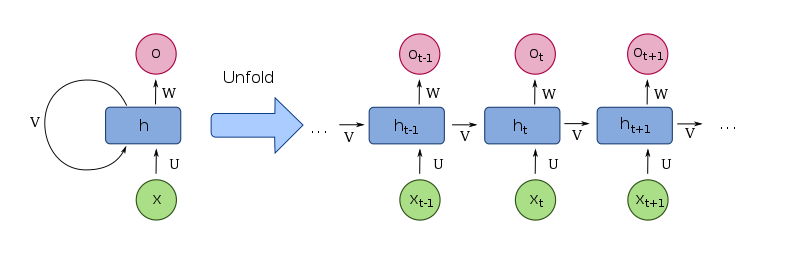
\includegraphics[width=0.7\textwidth]{Recurrent_neural_network_unfold.png}
    \caption[Recurrent Neural Networks Unfolded]{Recurrent Neural Networks Unfolded \cite{wiki:rnns}}
    \label{fig:4.1}
\end{figure}

Recurrent neural networks models contain a self-connected hidden layer. One benefit of the recurrent connection is that a `memory' of previous inputs remains in the network’s internal state, allowing it to make use of past context. This is significant for handwriting recognition as mentioned in \cite{art:ieee:consys}. A major problem with gradient descent for standard RNN architectures is that error gradients vanish exponentially quickly with the size of the time lag between important events \cite{wiki:rnns}.

\section{Long Short Term Memory}
\label{sec:lstm}

\textbf{Year:} 1997

Long short-term memory (LSTM) is a deep learning system that avoids the vanishing gradient problem. LSTM is normally augmented by recurrent gates called ``forget gates''. LSTM prevents backpropagated errors from vanishing or exploding. Instead, errors can flow backwards through unlimited numbers of virtual layers unfolded in space. That is, LSTM can learn tasks that require memories of events that happened thousands or even millions of discrete time steps earlier \cite{wiki:rnns}.

\begin{figure}[!htbp]
    \centering
    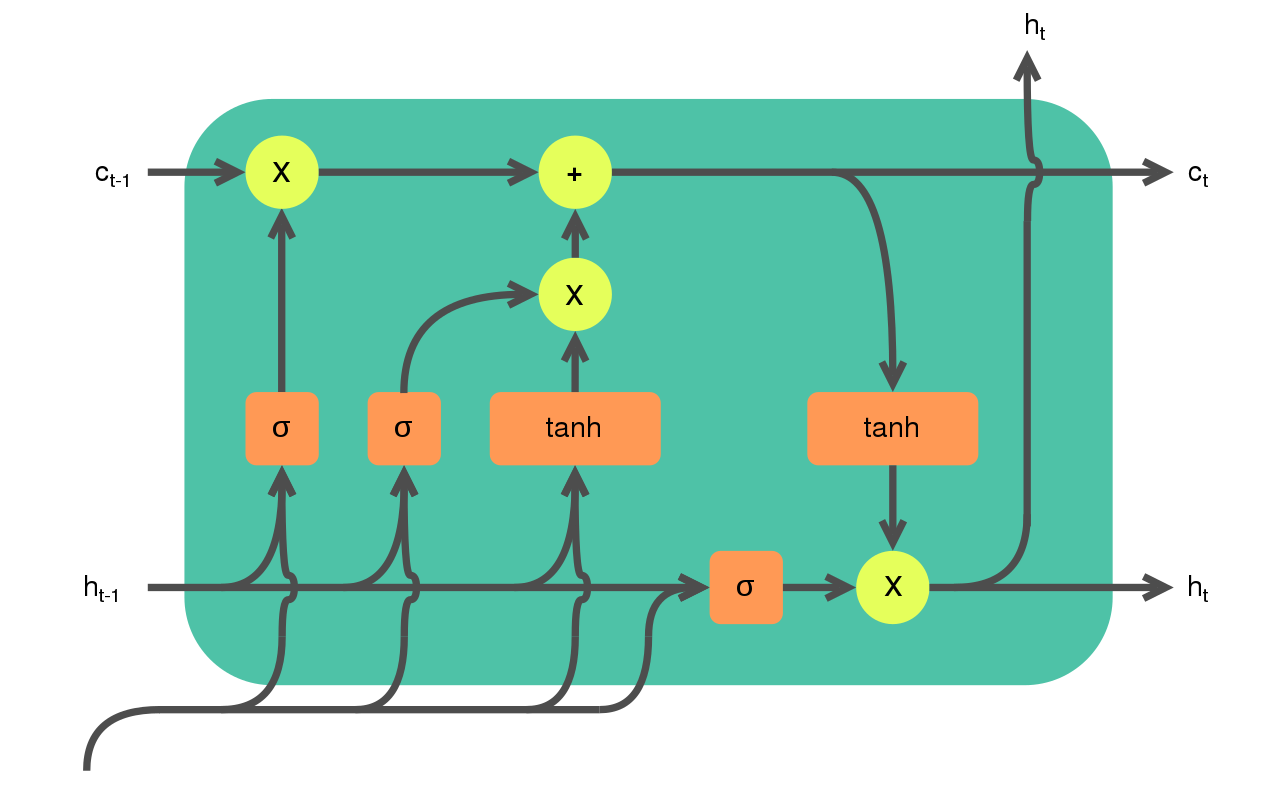
\includegraphics[width=0.7\textwidth]{LSTM_cell.png}
    \caption[Long Short Term Memory Cell]{Long Short Term Memory Cell \cite{wiki:lstm}}
    \label{fig:4.2}
\end{figure}

A common LSTM unit, as shown in figure \ref{fig:4.2}, is composed of a cell, an \emph{input gate}, an \emph{output gate} and a \emph{forget gate}. The cell remembers values over arbitrary time intervals and the three gates regulate the flow of information into and out of the cell. Some variations of the LSTM unit do not have one or more of these gates or maybe have other gates. For example, \emph{Gated Recurrent Units} (GRUs) do not have an output gate. LSTM networks are hence well-suited for classifying time series data.

The compact forms of the equations for the forward pass of an LSTM unit with a forget gate are:

\[f_t = \sigma_g(W_f x_t + U_f h_{t-1} + b_f)\]
\[i_t = \sigma_g(W_i x_t + U_i h_{t-1} + b_i)\]
\[o_t = \sigma_g(W_o x_t + U_o h_{t-1} + b_o)\]
\[\tilde{c}_t = \sigma_c(W_c x_t + U_c h_{t-1} + b_c)\]
\[c_t = f_t \circ c_{t-1} + i_t \circ \tilde{c}_t\]
\begin{equation}
    h_t = \sigma_t \circ \sigma_h(c_t)
\end{equation}

The initial values are $c_0 = 0$ and $h_0 = 0$ and the operator $\circ$ denotes the Hadamard element-wise product. Activations are $\sigma_g$ - a sigmoid function, $\sigma_c$ and $\sigma_h$  - a hyperbolic tangent functions. The variable are \cite{wiki:lstm}:

\begin{table}[h]
    \centering
    \begin{tabular}{ r l }
        $x_t$           : & input vector to the LSTM unit            \\
        $f_t$           : & forget gate's activation vector          \\
        $i_{t}$         : & input or update gate's activation vector \\
        $o_{t}$         : & output gate's activation vector          \\
        $h_{t}$         : & hidden state vector                      \\
        $\tilde{c}_{t}$ : & cell input activation vector             \\
        $c_{t}$         : & cell state vector
    \end{tabular}
\end{table}

\section{Convolution Neural Networks}
\label{sec:cnnlr}

\textbf{Year:} 1998

A convolutional neural network (CNN), is a class of deep neural networks, most commonly applied to analyzing visual imagery. They are also known as shift invariant or \emph{space invariant artificial neural networks} (SIANN). CNNs have a wide variety of applications including, image and video recognition, recommender system, brain-computer interface etc.

\begin{figure}[!htbp]
    \centering
    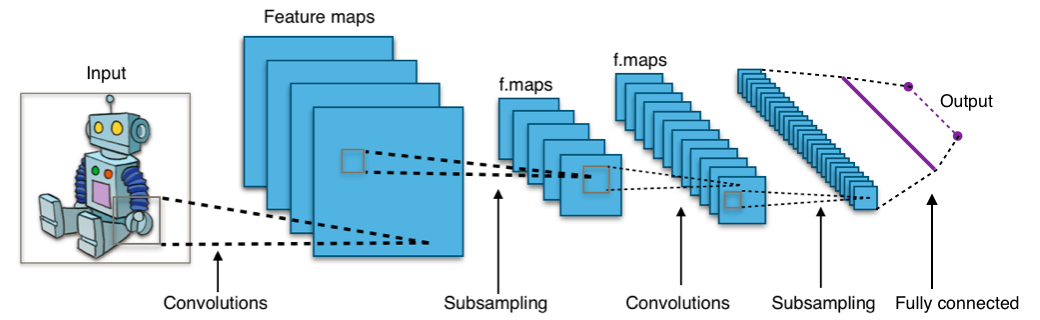
\includegraphics[width=0.7\textwidth]{Typical_cnn.png}
    \caption[Typical CNN Architecture]{Typical CNN Architecture \cite{wiki:cnns}}
    \label{fig:4.3}
\end{figure}

CNNs are regularized versions of multilayer perceptrons. Multilayer perceptrons usually mean fully connected networks, that is, each neuron in one layer is connected to all neurons in the next layer.

Convolutional networks were inspired by biological processes in that the connectivity pattern between neurons resembles the organization of the animal visual cortex. Figure \ref{fig:4.3} shows a common CNN architecture. CNNs use relatively less pre-processing compared to other image classification algorithms. Independence from prior knowledge and human effort in feature design is a major advantage \cite{wiki:cnns}. More about CNN in section \ref{sec:cnn}.

\section{The Transformer Network}
\label{sec:ttn}

\textbf{Year:} 2017

The Transformer is a deep learning model primarily used in the field of natural language processing (NLP). Transformers are designed to handle sequential data, such as natural language unlike RNNs, Transformers do not require that the sequential data be processed in order. Thus Transformer allows for much more parallelization than RNNs and therefore reduced training hours. This has led to the development of pre-trained systems such as BERT (Bidirectional Encoder Representations from Transformers) and GPT (Generative Pre-trained Transformer), which have been trained with huge general language datasets, and can be fine-tuned to specific language tasks.

Transformer is an encoder-decoder architecture. The \emph{encoder} consists of a set of encoding layers that processes the input iteratively one layer after another and the \emph{decoder} consists of a set of decoding layers that does the same thing to the output of the encoder. Each encoder and decoder layer makes use of an \emph{attention mechanism}, which for each input, weighs the relevance of every other input and draws information from them accordingly to produce the output. Each decoder layer also has an additional attention mechanism which draws information from the outputs of previous decoders, before the decoder layer draws information from the encodings. Both the encoder and decoder layers have a feed-forward neural network for additional processing of the outputs, and contain residual connections and layer normalization steps \cite{wiki:transformer}.

The basic building blocks of the Transformer are scaled dot-product attention units. When a sentence is passed into a Transformer model, attention weights are calculated between every token simultaneously. The attention unit produces embeddings for every token in context that contain information not only about the token itself, but also a weighted combination of other relevant tokens weighted by the attention weights. More about Transformer and Attention in section \ref{sec:vit}.
\vspace*{\fill}
%<<<<<<<<<<<<<<<<<<<<<<< Evolution <<<<<<<<<<<<<<<<<<<<<<<

%>>>>>>>>>>>>>>>>>>>>>>> Existing >>>>>>>>>>>>>>>>>>>>>>>
%>>>>>>>>>>>>>>>>>>>>>>> Existing >>>>>>>>>>>>>>>>>>>>>>>
\chapter{Concurrent Systems}
\label{chap:existing}
\thispagestyle{fancy}

\hspace{0.5cm} There are several existing systems or models which can perform digit recognition. Some of these even have state of the art accuracy claims. This section delves into two significant artificial neural network models, namely \emph{The Perceptron} and \emph{Convolutional Neural Network}. Even though these networks can perform a variety of tasks, the focus will be upon digit classification.

\section{Vanilla ANN - The perceptron}
\label{sec:perceptron}

\hspace{0.5cm} Vanilla Artificial Neural Network (ANN) is a primitive model. They are computing systems vaguely inspired by the biological neural networks. An ANN is based on a collection of connected units or nodes called artificial neurons, which loosely model the neurons in a biological brain. Each connection, like the synapses in a biological brain, can transmit a signal to other neurons.

\begin{figure}[!htbp]
    \centering
    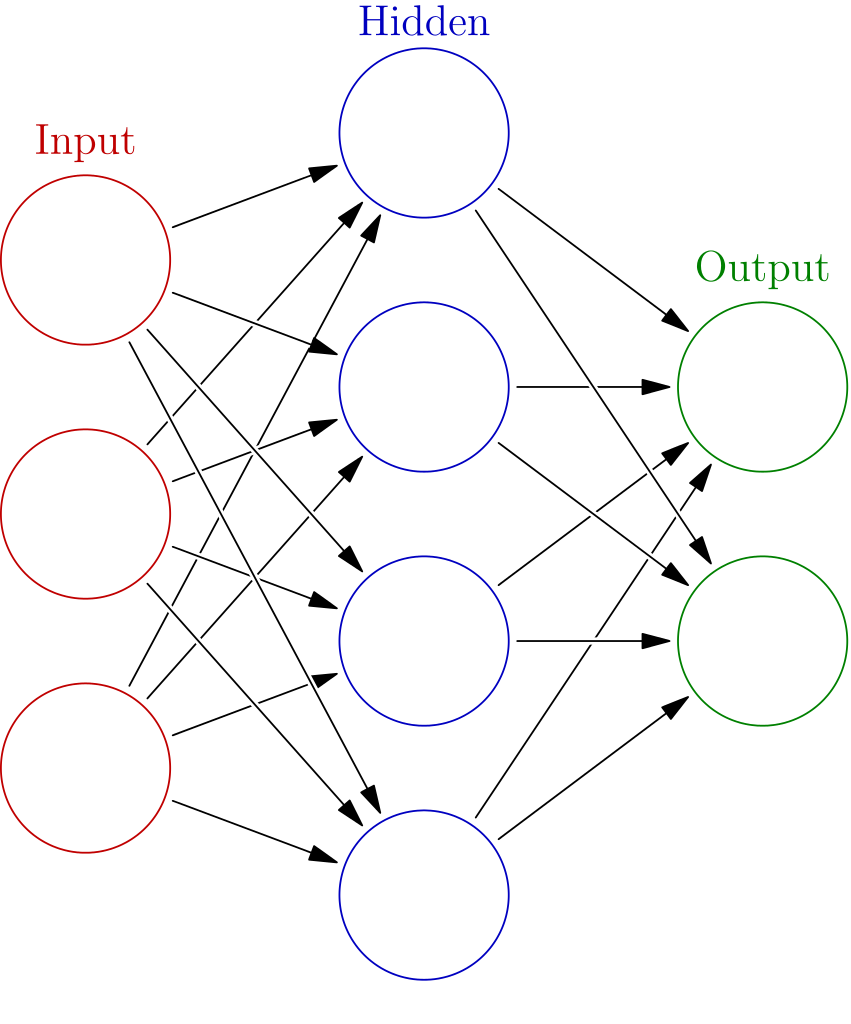
\includegraphics[height=0.5\textwidth]{artificial_neural_network.png}
    \caption[Simple Artificial Neural Network]{Simple Artificial Neural Network \cite{wiki:anns}}
    \label{fig:5.1}
\end{figure}

An artificial neuron that receives a signal then processes it and can signal neurons connected to it. The `signal' at a connection is a real number, and the output of each neuron is computed by some non-linear function of the sum of its inputs. The connections are called edges. Neurons and edges typically have a weight that adjusts as learning proceeds. The weight increases or decreases the strength of the signal at a connection. Neurons may have a threshold such that a signal is sent only if the aggregate signal crosses that threshold.

Typically, neurons are aggregated into layers. Different layers may perform different transformations on their inputs. Signals travel from the first layer (the input layer), to the last layer (the output layer), possibly after traversing the layers multiple times. \cite{wiki:anns}

\subsection{Neurons}
\label{subsec:neurons}
ANNs are composed of artificial neurons, each artificial neuron has inputs and produce a single output which can be sent to multiple other neurons. To find the output of the neuron, first we take the weighted sum of all the inputs, weighted by the weights of the connections from the inputs to the neuron. We add a bias term to this sum. This weighted sum is then passed through a (usually nonlinear) activation function to produce the output \cite{wiki:anns}.

\begin{figure}[!htbp]
    \centering
    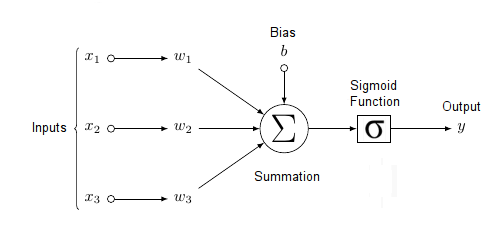
\includegraphics[width=0.7\textwidth]{artificial_neuron.png}
    \caption[Artificial Neuron]{Artificial Neuron}
    \label{fig:5.2}
\end{figure}

\subsection{Weights and Biases}
The network consists of connections, each connection providing the output of one neuron as an input to another neuron. Each connection is assigned a \emph{weight} $w_i$, that represents its relative importance. A given neuron can have multiple input and output connections. The \emph{activation} function $\sigma$, computes the input to a neuron from the outputs of its predecessor neurons and their connections as a weighted sum as shown in figure \ref{fig:5.2} A \emph{bias} $b$, term can be added to the result of the forward propagation \cite{wiki:anns}.

\begin{equation}
    \label{equ:5.1}
    a_i^{(j)} = \sigma(w_{i0}a_0^{(j)} + w_{i1}a_1^{(j)} + \hdots + w_{in}a_n^{(j)} + b_0)
\end{equation}

The equation \ref{equ:5.1} is an example of an output from a single layer, it can be generalized and expressed neatly as in \ref{equ:5.2}.

\begin{equation}
    \label{equ:5.2}
    a^{(L)} = \sigma(W^{(L)}a^{(L-1)} + b^{(L)})
\end{equation}

\subsection{Hyperparameters}
A hyperparameter is a constant parameter whose value is set before the learning process begins. The values of parameters are derived via learning. Examples of hyperparameters include learning rate, the number of hidden layers and batch size. The values of some hyperparameters can be dependent on those of other hyperparameters. For example, the size of some layers can depend on the overall number of layers \cite{wiki:anns}.

\subsection{Learning or Training}
Learning is the adaptation of the network to better handle a task by considering sample observations. Learning involves adjusting the weights (and optional thresholds) of the network to improve the accuracy of the result. This is done by minimizing the observed errors. Learning is complete when examining additional observations does not usefully reduce the error rate \cite{wiki:anns}.

\subsection{Backpropagation}
Backpropagation is a method to adjust the connection weights to compensate for each error found during learning. The error amount is effectively divided among the connections. Technically, Backpropagation calculates the gradient (the derivative) of the cost function associated with a given state with respect to the weights. The weight updates can be done via stochastic gradient descent or other methods \cite{wiki:anns}.

\subsection{Digit Recognition}
Since supervised model is used to create a a digit classifier, during the training dispensation the models is provided with correctly labeled outputs (say $y$). If errors arise, they need to be minimized. The cost function is calculated as the square of the difference between the expected and actual output.

\begin{equation}
    \label{equ:5.3}
    C_0 = (a^{(L)} - y)^2
\end{equation}

The RHS of \ref{equ:5.2} can re-written as $\sigma(z^{(L)})$. To minimize cost function the derivative needs to be found, and here chain rule can be applied:

\begin{equation}
    \label{equ:5.4}
    \frac{\partial C_0}{\partial w^{(L)}} = \frac{\partial z^{(L)}}{\partial w^{(L)}} \cdot \frac{\partial a^{(L)}}{\partial z^{(L)}} \cdot \frac{\partial C_0}{\partial a^{(L)}}
\end{equation}

Therefore for a single training sample the minimized cost function will be as in \ref{equ:5.5} and the net cost $\nabla C$ will be as shown in \ref{equ:5.7}.

\begin{equation}
    \label{equ:5.5}
    \frac{\partial C_0}{\partial w^{(L)}} = a^{(L-1)} \cdot \sigma'(z^{(L)}) \cdot 2(a^{(L)} - y)
\end{equation}

\begin{equation}
    \label{equ:5.6}
    \frac{\partial C}{\partial w^{(L)}} = \frac{1}{n} \sum_{k = 0}^{n - 1} \frac{\partial C_k}{\partial w^{(L)}}
\end{equation}

\begin{equation}
    \label{equ:5.7}
    \nabla C = \begin{bmatrix}
        \frac{\partial C}{\partial w^{(0)}} \\[1em]
        \frac{\partial C}{\partial w^{(1)}} \\[1em]
        \vdots                              \\[1em]
        \frac{\partial C}{\partial w^{(L)}}
    \end{bmatrix}
\end{equation}

This is propagated backwards, errors are minimised after each sample and hence the digits are recognized correctly \cite{yt:3b1b:nnp1}.

\section{Digit Recognition with CNN}
\label{sec:cnn}

\hspace{0.5cm} As stated in section \ref{sec:cnnlr}, digit recognition is a powerful deep learning model mostly used with digital image manipulation tasks. It is unsurprisingly complex, yet beautiful in construct. The accuracy with which CNNs classify object is at par. No wonder why the current SOTA holder is a CNN based model. This section tries to delve a little more deeper into what exactly CNNs does under the hood.

\subsection{Object Recognition Fundamentals}
\label{subsec:objrecfund}
General flow of digit recognition includes \cite{art:medium:hdreccnn}:
\begin{enumerate}
    \item \textbf{Image Acquisition :}  This stage receives an input image which can from in any format from any source. They can be of image formats like: .png, .jpeg or capture from a camera or scanner.
    \item \textbf{Preprocessing :} Here the input image undergoes a number of procedures which tries to minimize those factors which may cause the accuracy to drop. It usually works upon images to reduce and if possible remove distortions.
    \item \textbf{Segmentation :} It is used to isolate focused parts of the input. Histogram process is use retrieve the entities from the image. Contents are processed in a tree like structure.
    \item \textbf{Feature Extraction :} Converts an image into \emph{n-dimensional array tensor}. It extracts those features from the sample which are most importance for classification. Various techniques include Principle Component Analysis (PCA), Chain Code (CC) etc.
    \item \textbf{Classification :} Extracted characteristics is used to make decisions. Different classifier algorithms are used and they compare the input with the training sample. \emph{Softmax} regressions is applied to rate the accuracy in terms of probability.
    \item \textbf{Post Processing :} To correct misclassified results, shape recognition is used. Then along with the language knowledge, the errors can be minimized in case of handwriting recognition.
\end{enumerate}

\subsection{Demystifying CNNs}
\label{subsec:layrcnn}

\begin{figure}[!htbp]
    \centering
    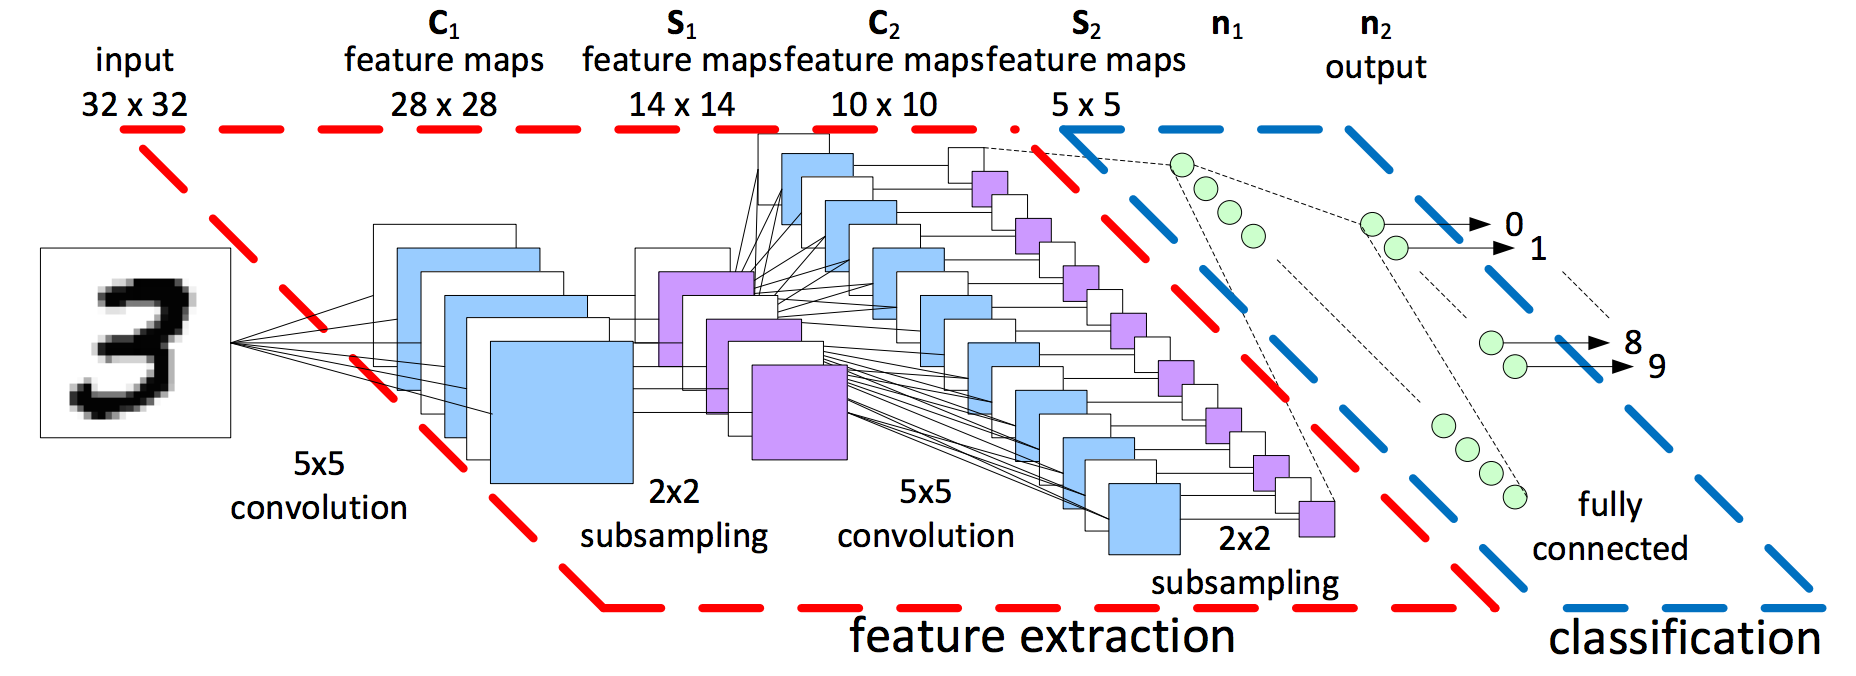
\includegraphics[width=0.7\textwidth]{cnn_layers.png}
    \caption[Layers in Convolutional Neural Network]{Layers in Convolutional Neural Network}
    \label{fig:5.3}
\end{figure}

\subsubsection{Tensor}
\label{subsub:tensor}

In mathematics, a tensor is an algebraic object that describes a (multilinear) relationship between sets of algebraic objects related to a vector space. Objects that tensors may map between, include vectors and scalars, and even other tensors. Tensors can take several different forms – for example: scalars and vectors etc \cite{wiki:tensor}.

\subsubsection{Convolution}
\label{subsub:convolution}

Convolutional layers convolve the input and pass its result to the next layer. The input is a tensor with shape (number of images) x (image height) x (image width) x (image depth). It becomes abstracted to a feature map, with shape (number of images) x (feature map height) x (feature map width) x (feature map channels) \cite{wiki:cnns}.

\subsubsection{Pooling}
\label{subsub:pooling}

Pooling layers reduce the dimensions of the data by combining the outputs of neuron clusters at one layer into a single neuron in the next layer. Local pooling combines small clusters, typically $2\times 2$. They are applied with a stride $S$, of 2 downsamples at every depth slice in the input by 2 along both width and height, discarding 75\% of the activations \cite{wiki:cnns}:

\begin{equation}
    \label{equ:5.8}
    f_{X,Y}(S) = \max_{a,b = 0}^1 S_{2X + a, 2Y + b}
\end{equation}

\subsubsection{Fully Connected Layer}
\label{subsub:fullycnlr}

Fully connected layers connect every neuron in one layer to every neuron in another layer. It is in principle the same as the traditional multi-layer perceptron neural network (MLP). The flattened matrix goes through a fully connected layer to classify the images \cite{wiki:cnns} and thus recognize handwritten digits aptly.

\section{Vision Transformer}
\label{sec:vit}

\hspace{0.5cm} On October 22, 2020 Google Research, Brain Team released an arXiv preprint on \emph{Vision Transformer} \cite{2020arXiv201011929D}. A paper on \emph{Image Transformer} was released in 2018 \cite{2018arXiv180205751P} which performed tasks like generative image modelling and super-resolution scaling. The latter model as expected diverted to fulfill different purpose. Inspired by the Transformer scaling successes in NLP, \cite{2020arXiv201011929D} experiments with applying a standard Transformer \cite{2017arXiv170603762V} directly to images, with the fewest possible modifications.

\subsection{ViT Architecture}

\begin{figure}[!htbp]
    \centering
    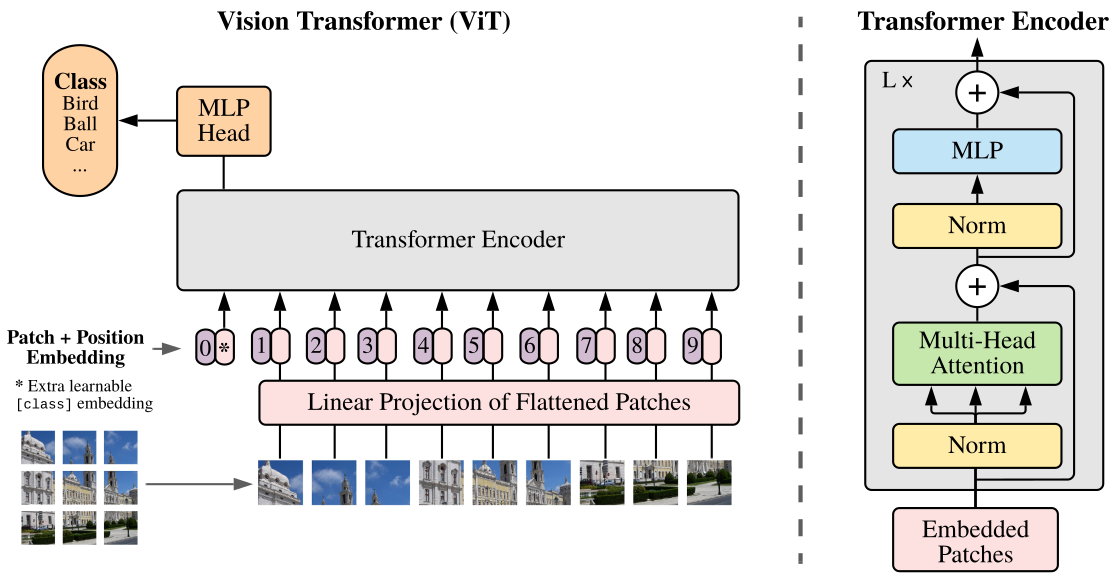
\includegraphics[width=0.7\textwidth]{vision_transformer.png}
    \caption[Vision Transformer Architecture]{Vision Transformer Architecture \cite{2020arXiv201011929D}}
    \label{fig:5.4}
\end{figure}

The input image is split into fixed-size patches and each one of them is linearly embedded and position embeddings are added. The resulting sequence of vectors is fed to a standard Transformer
encoder \cite{2017arXiv170603762V}. In order to perform classification, ViT uses the standard approach of adding an extra learnable `classification token' to the sequence.

The standard Transformer receives as input a 1D sequence of token embeddings. To handle 2D images, image $x \in \mathbb{R}^{H\times W\times C}$ is reshaped into a sequence of flattened 2D patches $x_p \in \mathbb{R}^{N\times (P^2 \cdot C)}$ where:

\begin{itemize}
    \item $(H, W)$ is the resolution of original image,
    \item $C$ is the number of channels
    \item $(P, P)$ is the resolution of each image patch and
    \item $N = HW/P^2$ is the resulting number of patches.
\end{itemize}

The Transformer uses constant latent vector size $D$ throughout all of it layers fo the flatten patches are mapped to $D$ dimensions, with a trainable linear projection. This is termed as \emph{patch embeddings}. A learnable embedded is pre-appended to the sequence embedding, whose state at the output of the Transformer encoder $(\textbf{z}_L^0)$ serves as the image representation $y$. Both during pre-training and fine-tuning, a classification head is attached to $(\textbf{z}_L^0)$. The classification head is implemented by a Multi-layer Perceptron (MLP) with one hidden layer at pre-training time and by a single linear layer at fine-tuning time \cite{2020arXiv201011929D}.

\subsection{Hybrid Architecture}
\label{subsec:hybrdarch}

\hspace{0.5cm} As an alternative to raw image patches, the input sequence can be formed from feature maps of a CNN \cite{art:ieee:backprophzcr}. In this hybrid model, the patch embedding projection is applied to patches extracted from a CNN feature map. As a special case, the patches can have spatial size $1\times 1$, which means that the input sequence is obtained by simply flattening the spatial dimensions of the feature map and projecting to the Transformer dimension. The classification input embedding and position embeddings are added as described above \cite{2020arXiv201011929D}.

\subsection{Fine Tuning ViT}
\label{subsec:finevit}

\hspace{0.5cm} Typically, ViT is pre-trained on large datasets, and fine-tuned to (smaller) downstream tasks. For this, the pre-trained prediction head is removed and a zero-initialized $D\times K$ feed-forward layer is attached, where $K$ is the number of downstream classes. It is often beneficial to fine-tune at higher resolution than pre-training. When feeding images of higher resolution, the patch size is kept the same, which results in a larger effective sequence length. The Vision Transformer can handle arbitrary sequence lengths (up to memory constraints), however, the pre-trained position embeddings may no longer be meaningful. Therefore 2D interpolation of the pre-trained position embeddings is performed, according to their location in the original image \cite{2020arXiv201011929D}.
\vspace*{\fill}
%<<<<<<<<<<<<<<<<<<<<<<< Existing <<<<<<<<<<<<<<<<<<<<<<

%>>>>>>>>>>>>>>>>>>>>>>> Proposed >>>>>>>>>>>>>>>>>>>>>>>
%>>>>>>>>>>>>>>>>>>>>>>> Proposed >>>>>>>>>>>>>>>>>>>>>>>
\chapter{Proposed System}
\label{chap:proposed}
\thispagestyle{fancy}

\hspace{0.5cm} We've so far approached the project from machine learning perspective. Being a research oriented project, it focuses on the field of digit recognition. Yet to remind the reader about another part which is as relevant - is to solve sudoku. Sudoku is a known mathematical game by nearly each a every person on the plant. So initially it might sound simple and that is quite natural as our cognitive thinking skills tackles a problem with vigorous intuitiveness. But a machine needs to be told to solve a task in the sequence of steps, which is called an algorithm.

Various algorithms exists to solve sudoku, some of which are `backtracking', `stochastic search', `exact cover' and `constrain programming' \cite{wiki:solvsdkalgo}. This project can be said to have two broad parts - \emph{Artificial Intelligence} and \emph{Sudoku Solver}. Figure \ref{fig:6.1} showcases an overly simplified project logic.

\begin{figure}[!htbp]
    \centering
    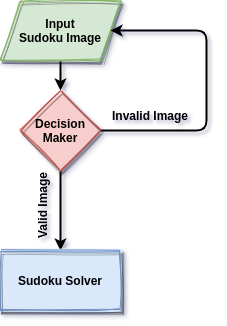
\includegraphics[height=0.5\textwidth]{vudoku_arch01.png}
    \caption[Vudoku: Simplified Architecture]{Vudoku: Simplified Architecture}
    \label{fig:6.1}
\end{figure}

The fundamental idea is to capture sudoku pattern from images (even handwritten ones) using the latest Vision Transformer and solve them by an effective algorithm.

\section{Project Modules}
\label{sec:prjtmod}

\hspace{0.5cm} It is always recommended to approach a problem part by part. Following the divide and conquer method

\subsection{Sudoku Algorithm(s)}
\label{subsec:sdkalgo}

\subsection{Implementation and Analysis}
\label{subsec:implmnt}
\vspace*{\fill}
%<<<<<<<<<<<<<<<<<<<<<<< Proposed <<<<<<<<<<<<<<<<<<<<<<<

%>>>>>>>>>>>>>>>>>>>>>>> Conclusion >>>>>>>>>>>>>>>>>>>>>>>
%>>>>>>>>>>>>>>>>>>>>>>> Conclusion >>>>>>>>>>>>>>>>>>>>>>>
\chapter{Conclusion}
\label{chap:conclusion}
\thispagestyle{fancy}
\vspace*{\fill}
%<<<<<<<<<<<<<<<<<<<<<<< Conclusion <<<<<<<<<<<<<<<<<<<<<<<

\bibliographystyle{unsrt}
\bibliography{references}
\thispagestyle{fancy}

\end{document}